
\section{Comparison on Benchmarks}
This section presents a comparison between linear Dec-ODE and state-of-the-art methods using standard benchmarks.

\subsection{Experiment Setup \label{sec:experimentSetup}}
\label{sec:setup}

\textbf{Datasets.}  
We evaluated our approach on five widely-used real-world datasets from various domains:  
{\bf Reddit} represents sequences of social media posts,  
{\bf Stack Overflow (SO)} comprises sequences of rewards from the question-answering platform,  
{\bf MIMIC-II} contains sequences of diagnoses from clinical visits to the Intensive Care Unit (ICU),  
{\bf MOOC} includes sequences of user interactions with an online course,  
and {\bf Retweet} captures sequences of social media posts. Detailed descriptions of these datasets are provided in the Sec. \ref{sec:data-desc}.  
To ensure comparability across results, all time points were normalized by the standard deviation of the time gaps, $\{t_i - t_{i-1}\}_{i=1}^n$, within the training set, following the procedure outlined in \cite{bib:MetaTPP}.  

\textbf{Metrics.}  
We employed three conventional metrics for evaluation:  
1) \textit{Negative Log-Likelihood} (NLL) assesses the suitability of the predicted probability density, as computed via \eqref{eq:obj};  
2) \textit{Root Mean Squared Error} (RMSE) evaluates the accuracy of predicted event time points;  
3) \textit{Accuracy} (ACC) quantifies the correctness of the predicted mark distribution $f^*(k|t)$.  
For predictions, the expected value $\mathbb{E}_{f^*}[t]$ was used as the predicted time of the next event, and the mark with the highest probability at time $t$, i.e., $\argmax(f^*(k|t))$, was selected as the predicted mark.  

\textbf{Baseline.}  
We compared our method against four state-of-the-art approaches:  
Recurrent Marked Temporal Point Process (RMTPP) \cite{bib:RMTPP}, Transformer Hawkes Process (THP) \cite{bib:THP}, Intensity-Free Learning (IFL) \cite{bib:ifl}, and Attentive Neural Hawkes Process (ANHP) \cite{bib:ANHP}.  
Both THP and ANHP are transformer-based models that utilize the full set of observed events $\mathcal{H}_{t_n}$ to predict $e_{n+1}$.  
IFL directly models $f^*(t,k) = f^*(t) f^*(k|t)$ using a log-normal mixture for a more flexible distribution.  
As it explicitly parameterizes the distribution $f^*(t)$, the expected value $\mathbb{E}_{f^*}[t]$ can be computed analytically.  
Additional implementation details are provided in Sec.\ref{sec:baselineImplementation}.


\begin{table}[!t]
\centering
\caption{Comparison with the state of the art methods on 5 popular real-life datasets. Results with \textbf{boldface} and \underline{underline} represent the best and the second-best results, respectively. Following \cite{bib:THP, bib:ANHP} the mean and std are gained by bootstrapping 1000 times.}
\renewcommand{\arraystretch}{1.3}
\small
\scalebox{0.52}[0.52]{

\begin{tabular}{c | c c c c | c | c c c c | c | c c c c | c} 
& \multicolumn{5}{c|}{RMSE} & \multicolumn{5}{c|}{ACC} & \multicolumn{5}{c}{NLL}\\
\cline{2-6} \cline{7-11} \cline{12-16}
&  RMTPP & THP & IFL & ANHP & \textbf{Dec-ODE} & RMTPP & THP & IFL & ANHP & \textbf{Dec-ODE} & RMTPP & THP & IFL & ANHP & \textbf{Dec-ODE}\\ 
\hline
\hline
\multirow{2}{*}{MOOC} & $0.473$ & $0.476$ & $0.501$ & \underline{$0.470$} & $\textbf{0.467}$
                        & $20.98$ & $24.49$ & $\underline{32.30}$ & $31.53$ & $\textbf{42.08}$ 
                        & $-0.315$ & $0.733$ & $\textbf{-2.895}$ & $\underline{-2.632}$ & $-2.289$  \\  [-3pt]
                    & ${(0.012)}$ & $(0.010)$ & ${(0.012)}$ & $\underline{(0.019)}$ & $\textbf{(0.012)}$
                    & $(0.29)$ &${(0.22)}$ & $\underline{(1.30)}$ & $(0.20)$ & $\textbf{(0.44)}$
                    & $(0.031)$ & $(0.047)$ & $\textbf{(0.031)}$ & $(\underline{0.043})$ & ${(0.191)}$ \\[3pt]
\multirow{2}{*}{Reddit} & $\underline{0.953} $ & $6.151$ & $1.040$ & $1.149$ & $\textbf{0.934}$
                        & $29.67$ & $60.72$ & $48.91$ & $\textbf{63.45}$ & $\underline{62.32}$ 
                        & $3.559$ & $2.335$ & $2.188$ & $\textbf{1.203}$ & $\underline{1.367}$ \\[-3pt]
                        & $\underline{(0.016)}$ & $(0.195)$ &  $(0.017)$ & $(0.010)$ & $\textbf{(0.017)}$
                        & $(1.19)$ & $(0.08)$ & $(1.27)$ & $\textbf{(0.16)}$ & $\underline{(0.11)}$ 
                        & $(0.070)$ &$(0.031)$ & $(0.088)$ & $\textbf{(0.068)}$ & $\underline{(0.126)}$ \\[3pt]
\multirow{2}{*}{Retweet} & $\underline{0.990} $ & $1.055$ & $1.012$ & $1.663$ & $\textbf{0.985}$ 
                        & $51.72$ & $\textbf{60.68} $ & $55.35$ & ${59.72}$ & $\underline{60.17}$ 
                        & $-2.180$ & $-2.597$ & $-2.672$ & $\textbf{-3.134}$ & $\underline{-2.897}$ \\[-3pt]
                    & $\underline{(0.016)}$ & $(0.015)$ & $(0.018)$ & $(0.014)$ & $\textbf{(0.016)}$
                    & $(0.33)$ & $\textbf{(0.11)}$ & $(0.19)$ & $(0.11)$ & $\underline{(0.23)}$ 
                    & $(0.025)$ & $(0.016)$ & $(0.023)$ & $\textbf{(0.019)}$ & $\underline{(0.030)}$ \\[3pt]
\multirow{2}{*}{MIMIC-II} & $\underline{0.859} $ & $>10$ & $1.005$ & $0.933$ & $\textbf{0.810}$ 
                        & $78.20$ & $\textbf{85.98} $ & $80.49$ & $84.30$ & $\underline{85.06}$ 
                        & $1.167$ & $5.657$ & $\textbf{0.939} $ & $\underline{1.025}$ & $1.354$ \\  [-3pt]
                    & $\underline{(0.093)} $ & $(0.114)$ & $(0.121)$ & $(0.088)$ & $\textbf{(0.173)}$
                    & $(5.00)$ & $\textbf{(2.56)} $ & $(5.20)$ & $(2.78)$ & $\underline{(3.65)}$ 
                    & $(0.150)$ & $(0.304)$ & $\textbf{(0.139)} $ & $\underline{(0.155)}$ & $(0.413)$ \\[3pt]
\multirow{2}{*}{} \text{Stack} & $\textbf{1.017} $ & $1.057$ & $1.340$ & $1.052$ & $\underline{1.018}$
                    & $53.95$ & $53.83$ & $53.00$ & $\textbf{56.80}$ & $\underline{55.58}$ 
                    & $2.156$ &$2.318$ & $2.314$ & $\textbf{1.873}$ & $\underline{2.063}$  \\ [-3pt]
                    \text{Overflow} &  $\textbf{(0.011)}$ & $(0.011)$ & $(0.013)$ & $(0.011)$ & $\underline{(0.011)}$
                    & $(0.32)$ & $(0.18)$ & $(0.35)$ & $\textbf{(0.18)} $ & $\underline{(0.29)}$ 
                    & $(0.022)$ & $(0.022)$ & $(0.020)$ & $\textbf{(0.017)} $ & $\underline{(0.016)}$     \\[3pt]
                    \hline
\end{tabular}}
\label{table: real-life}
\end{table}

\subsection{Comparison of Results}
\label{sec: real-life}

We evaluate the performance of linear Dec-ODE against state-of-the-art TPP methods using the five real-world datasets described in Sec. \ref{sec:setup}. A summary of the results is provided in Table \ref{table: real-life}.  
Overall, our approach achieved results that were comparable to or better than the baselines across all metrics.  
This demonstrates that Dec-ODE effectively captures the complex dynamics of MTPPs through independently propagated influence functions.  
Notably, Dec-ODE excelled in prediction tasks, as evidenced by its low RMSE, while ANHP slightly outperformed it in NLL. Additionally, methods like Dec-ODE and IFL, which estimate $f^*(t)$ to compute $\mathbb{E}[t]$, tended to predict event times more accurately.  

\textbf{Discussion.}  
To ensure a fair comparison, we increased the number of samples used in the thinning algorithm \cite{lec:thinning, bib:thinning_ogata} implemented by \cite{bib:ANHP}. In most cases, the sample count was increased by a factor of 20. However, on the Reddit dataset with THP, the thinning algorithm struggled to sample correctly from $f^*(t)$ due to the low magnitude and high fluctuation of the intensity function. Additional details are provided in Sec.\ref{appen: thinning}.

\subsection{Explainability of Dec-ODE\label{exp: explainability}}

In MTPP and TPP, events have a temporal and complex influence on $\lambda^*(t)$ and $f^*(t)$ \cite{bib:hawkesOrigin, ISHAM1979335}.  
Thus, when evaluating the explainability of a neural network modeling an MTPP, it is crucial to understand how individual events impact predictions and how these effects evolve over time.  
Dec-ODE inherently provides this information.  
For instance, the temporal behavior of $\lambda_g^*(t)$ and $\hat{f}^*(k|t)$ can be directly visualized, as shown in Fig. \ref{fig: so fk}.

\begin{wrapfigure}{r}{0.40\textwidth}
    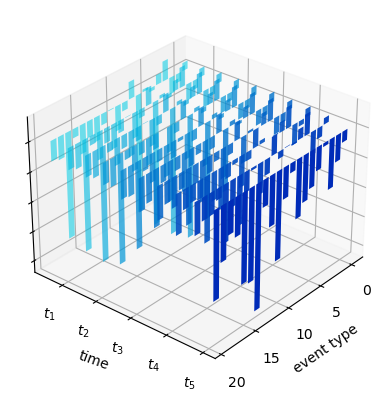
\includegraphics[width=0.92\linewidth, height=5cm]{figure/fk_dynamic.png}
    \captionsetup[figure]{font=small, justification=justified, margin=0.1cm}
    \captionof{figure}{Visualization of propagated $\hat{f}^*(k|t, e_i)$ in the StackOverflow experiment. The axes represent time, event type, and magnitude, respectively.}
    \label{fig: so fk}
\end{wrapfigure}

Our detailed analysis of the Retweet dataset further corroborates Dec-ODE's explainability.  
For example, meaningful patterns in the Retweet data are visualized in Fig. \ref{fig:retweet pattern}.  
The dataset comprises three classes:  
a post by a user with few followers ($\sim50\%$ of the population),  
a post by a user with a moderate number of followers ($\sim45\%$),  
and a post by a user with many followers ($\sim5\%$), labeled as 0, 1, and 2, respectively.  
In Fig. \ref{fig:retweet_inten}, which visualizes $\mu(t; e_i)$ conditioned on different $e_i$, each event shows a temporally decaying influence on $\lambda_g(t)$.  
This aligns with the expected behavior of social media posts, which generally elicit immediate reactions rather than delayed effects. 
Moreover, posts from users with many followers exhibit slower decay, as they tend to have broader exposure and sustain their influence for a longer time.

\begin{figure}
    \centering
    \subfigure[Influence function $\mu(t)$ conditioned on different event types, plotted over the same time range.]{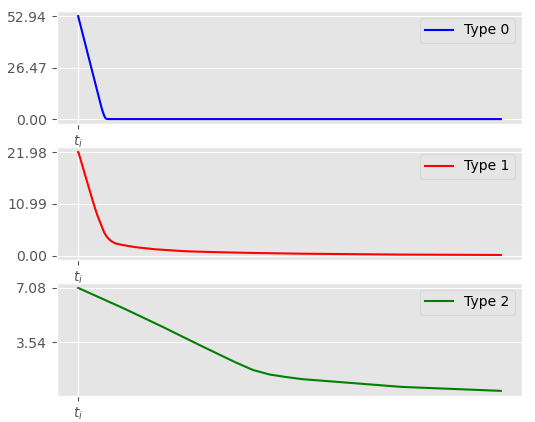
\includegraphics[width=0.46\linewidth, height=50mm]{figure/retweet_int.png} \label{fig:retweet_inten}} \hspace{5mm}
    \subfigure[Averaged influence proportions between different marks.]{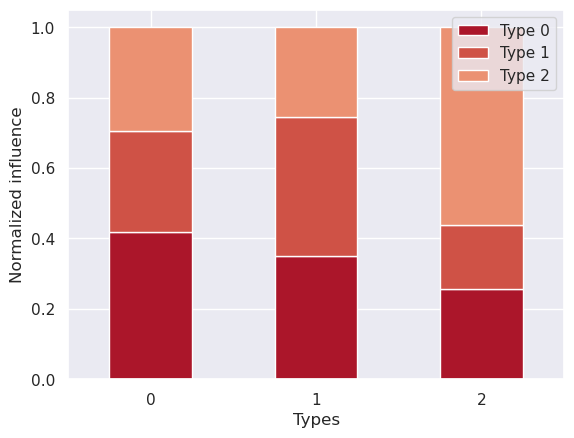
\includegraphics[width=0.46\linewidth, height=50mm]{figure/retweet_bar.png} \label{fig:retweet_bar}}
    \subfigure[Visualization of event marks over time. Blue (0): users with few followers, Red (1): users with moderate followers, Green (2): users with many followers.]{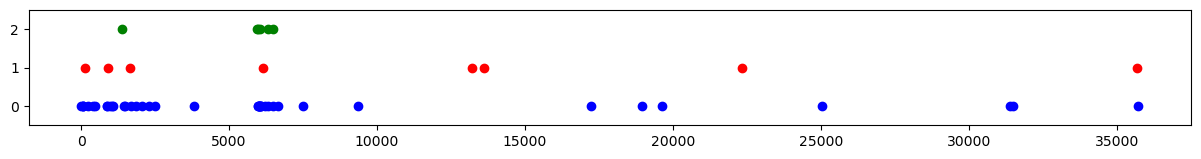
\includegraphics[width=0.95\linewidth]{figure/retweet_dot.png} \label{fig:retweet_dot}}
    \caption{\small Visualization of patterns in the Retweet dataset. (a) $\mu(t; e_i)$ for different marks, (b) Interaction between marks, (c) Event marks over time.}
    \label{fig:retweet pattern}
\end{figure}

Furthermore, the averaged proportions of influence across different mark types are shown in Fig. \ref{fig:retweet_bar}.  
First, despite type 2 accounting for only $5\%$ of the population, it exerts significant influence on the overall occurrence of events.  
This is consistent with the notion that individuals with many followers tend to impact a larger audience.  
Second, events of the same type have the strongest mutual influence.  
Given the exponentially decaying pattern of $\mu(t)$ and the large initial influence magnitude of type 0 (Fig. \ref{fig:retweet_inten}), events of type 0 likely exhibit strong clustering.  
This inference is validated by the visualization in Fig. \ref{fig:retweet_dot}.



\subsection{Parallel Computing Scheme \label{ablation: parallel}}
While Neural ODEs are highly effective at learning the continuous dynamics of a system, propagating the hidden state requires solving the IVP step by step, which can be computationally intensive.  
In Sec. \ref{train_parallel}, we introduced a method to propagate the hidden state through time in parallel by disentangling individual events.  
We validate this optimization scheme by comparing the average iteration time with that of traditional IVP-based sequential propagation.  

For the sequential approach, the differential equation is solved incrementally from $t_0$ to $t_n$.  
Table \ref{tab:parallel} presents the results, demonstrating a significant reduction in computation time across all cases.  
The parallelized computation for Dec-ODE was at least twice as fast (e.g., for MIMIC-II) and up to five times faster (e.g., for Reddit) compared to the traditional sequential scheme.

\begin{table}[h]
\renewcommand{\arraystretch}{1.1}
\centering
\caption{Training efficiency comparison in different datasets with the average time taken for an iteration (sec/iter) as the metric. Ratio shows that the iteration time at least reduces in half.}
\scalebox{0.6}[0.6]{
\begin{tabular}{cc |c| cc|c | c c|c | cc|c } 
\multicolumn{3}{c|}{StackOverflow} & \multicolumn{3}{c|}{MIMIC-II} & \multicolumn{3}{c|}{Retweet} & \multicolumn{3}{c}{Reddit}\\[-2pt]
\hline
parallel &Sequential& Ratio &  parallel& Sequential&Ratio &  parallel&Sequential&Ratio &  parallel&Sequential&Ratio\\
\hline
\multirow{1}{*}{} $15.0$ & $57.7$ &0.26 & $2.9$ & $6.5$ & $0.47$ & $16.8$ & $67.6$ &$0.25$ & $15.5$ & $78.7$ & $0.20$ \\
   
\end{tabular}
}
\label{tab:parallel}
\end{table}


\section{Linear vs. Non-Linear Influence Function\label{lin-nonlin}}  
In Table \ref{table: real-life}, the basic Dec-ODE model with a linear $\Phi_\lambda$ was evaluated.  
However, both $\Phi_\lambda$ and $\Phi_k$ can be defined as any functions, including neural networks, as long as they meet the conditions outlined in Secs. \ref{sec:ground int} and \ref{sec:fk}.  
Notably, with a linear $\Phi_\lambda$, every influence function must satisfy $\mu(t) \ge 0$ to ensure the intensity remains positive.  
This constraint means that only excitatory effects, where events increase the intensity, can be modeled.  

In this section, we explore the extensibility of our framework by introducing and testing a less restricted variant, referred to as the \textit{non-linear} $\Phi_\lambda$.  
The non-linear $\Phi_\lambda(t)$ is defined as follows:

\begin{align}
    \Phi_\lambda(\mu(t;e_0), \cdots, \mu(t;e_i)) = \text{softplus} \bigg( \sum _{e_i \in \mathcal{H}_{t}}  \mu  (t; e_i) \bigg).
\end{align}

Through this modeling approach, inhibitory effects, where an event reduces the overall intensity, can be incorporated.

To assess how this relaxation influences the modeling of TPP, both linear and non-linear models are tested in a simplified setting, using only the first 40 events from each sequence. The experimental results are summarized in Table \ref{tab:nonlin}, with NLL as the evaluation metric.  
In most cases, the overall result regarding the ground intensity improved, indicating that a more flexible $\Phi_\lambda$ allows for a more accurate prediction of the intensity function.

However, the non-linear Dec-ODE model reveals limitations when predicting time-delayed effects, where an event does not immediately influence the intensity but instead has a delayed effect. This issue arises because the inhibitory effect outweighs the excitatory one, causing the intensity function to drop to zero. In such situations, the inhibitory effect hinders the model's performance.

In conclusion, this experiment suggests that a more flexible $\Phi_\lambda$ can lead to higher fidelity predictions in most cases. However, further discussion is needed regarding the introduction of constraints to more effectively model various patterns in TPP.


\begin{table}[h]
\centering
\caption{Experiment on non-linear $\Phi_\lambda$. The softplus is applied after the summation in order to express inhibitory effects.}
\scalebox{0.9}[0.9]{
\begin{tabular}{cc | cc| c c | cc } \Xhline{0.3ex}
\multicolumn{2}{c|}{StackOverflow} & \multicolumn{2}{c|}{MIMIC-II} & \multicolumn{2}{c|}{Retweet} & \multicolumn{2}{c}{Reddit}\\[-2pt]
Linear & Non-linear &  Linear & Non-linear  &  Linear & Non-linear  & Linear & Non-linear\\
\hline
\multirow{1}{*}{} $0.9948$ & $\textbf{0.8987}$ &0.2451 & $\textbf{0.2183}$ & $-5.0872$ & $\textbf{-5.1649}$ & $\textbf{0.5163}$ & $18.2571$ \\
\Xhline{0.3ex}      
\end{tabular}}
    \label{tab:nonlin}
\end{table}

\section{Imputation \label{appen:imputation}}
In this section, we explore the impact of independently modeling hidden state dynamics by comparing it with methods that utilize contextual information. 
To examine this, events from the StackOverflow dataset are randomly removed to observe how the behavior changes as the number of observed events decreases.

\setlength{\intextsep}{0pt}
\begin{wrapfigure}{r}{0.46\textwidth}
    \centering
    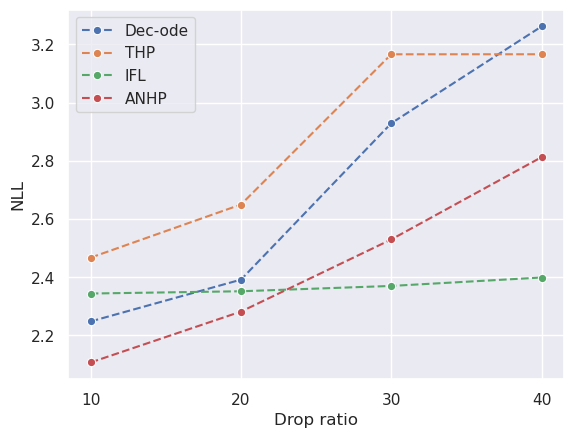
\includegraphics[width=0.44\textwidth]{figure/imputation.png}
    \caption{\raggedright Imputation experiment done using Stackoverflow dataset, where from $10\%$ to $40\%$ of data are randomly dropped.}  
    \label{fig:imputation}
\end{wrapfigure} 

For a fair comparison, we randomly selected 90\%, 80\%, 70\%, and 60\% of the indexes from the test dataset, and saved the corresponding data as new test sets. 
The results using these new test sets are visualized in Figure \ref{fig:imputation}.
The graph shows that the performance decline of Dec-ODE follows a similar trend when compared to other methods.

This suggests that the other methods are unable to recover from the loss of information. 
This conclusion is supported by the fact that Dec-ODE, which does not account for inter-event relationships, exhibits a similar trend.

\clearpage
\section{Simulation Study}


    \begin{figure}[!h]
        \centering
        \subfigure[]{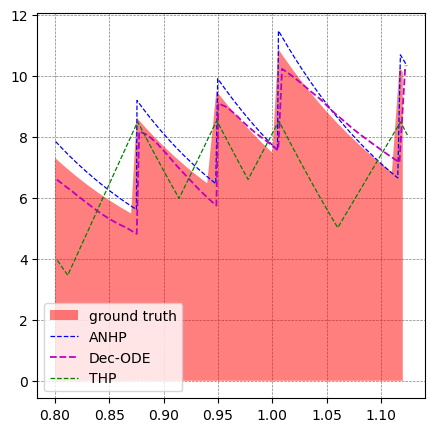
\includegraphics[height = 0.3\linewidth]{figure/total_intensity1.png}\label{fig:sim_a}}\hspace{-1mm}
        \subfigure[]{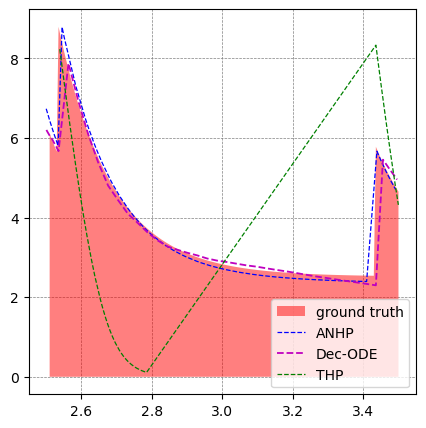
\includegraphics[height = 0.3\linewidth]{figure/total_intensity2.png}\label{fig:sim_b}}\hspace{-1mm}
        \subfigure[]{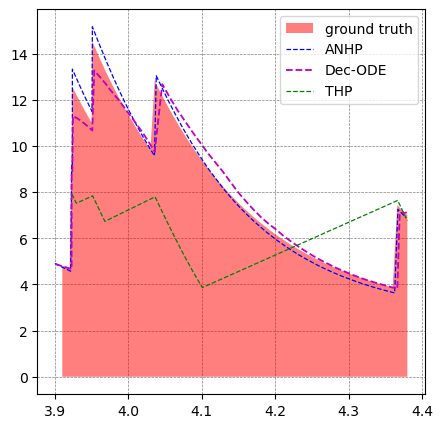
\includegraphics[height = 0.3\linewidth]{figure/total_intensity3.png}\label{fig:sim_c}}\hspace{-1mm}
        \subfigure[]{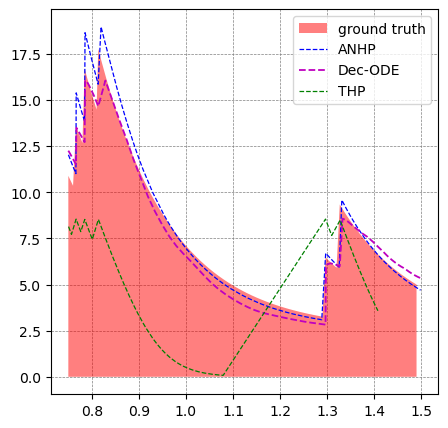
\includegraphics[height = 0.35\linewidth]{figure/total_intensity4.png}\label{fig:sim_d}}\hspace{1mm}
        \subfigure[]{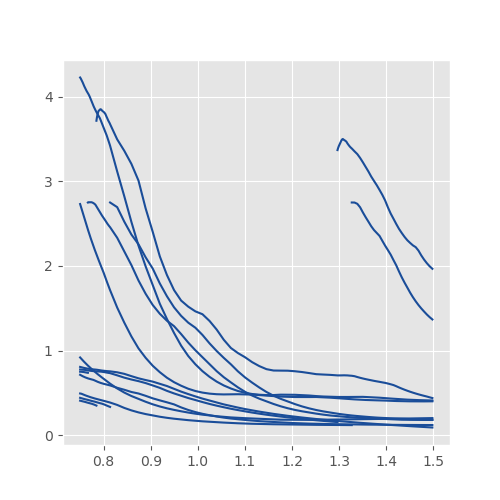
\includegraphics[height = 0.4\linewidth]{figure/decoupled_intensity4.png}\label{fig:sim_ae}}\hspace{1mm}
        \caption{Visualization from a simulation study. (a), (b), (c), and (d) compare the true intensity function of a Hawkes process and the reconstructed results from THP, ANHP, and Dec-ODEs. Each $\mu(t)$ that composes the result in (d) is illustrated in (e).}
        \label{fig:simulation}
    \end{figure}
    
    \begin{table}[h]
        \centering
        \begin{tabular}{c|c|c|c}
                & RMSE   & ACC   & NLL    \\ \hline
        THP     & 0.7734 & 27.48 & 3.0121 \\ 
        ANHP    & 0.6528 & 30.31 & 0.2807 \\ 
        Dec-ODE & \textbf{0.6568} & \textbf{30.35} & \textbf{0.2739} 
        \end{tabular}
        \caption{Estimation accuracy on the simulated Hawkes process. }
            \label{tab:simulation}
        \end{table}

We conducted a simulation study on the Hawkes process, following a similar procedure to that of the Neural Hawkes Process (NHP) \cite{bib:nhp}. 
To obtain the true intensity function, we randomly sampled parameters for the kernel function of the multivariate Hawkes process and simulated synthetic data using the tick library \cite{bacry2018tick}. 
The sampling range was adjusted from the NHP due to differences in scale between the library and the original paper.
In Figures \ref{fig:sim_a} - \ref{fig:sim_d}, THP struggles to capture the flexible dynamics of the intensity function $\lambda_g$, while ANHP and Dec-ODE exhibit dynamics closely resembling the ground truth intensity. 
Table \ref{tab:simulation} further shows that Dec-ODE outperforms both THP and ANHP across all metrics. 
These results align with those in Table \ref{table: real-life}, suggesting that Dec-ODE is capable of reliably simulating MTPPs compared to other state-of-the-art methods. 
Figure \ref{fig:sim_ae} visualizes $\mu(t)$ components that make up $\lambda_g(t)$ from Figure \ref{fig:sim_d}, demonstrating that the ground intensity $\lambda_g(t)$ can be reconstructed from the individually modeled trajectories, i.e., an MTPP can be effectively modeled using decoupled information.


\section{Train time comparison}

The time required for training one epoch (sec / epoch) is measured in order to compare the time required for training. 
The experiment is conducted using a single NVIDIA RTX A6000 GPU (48GB memory) with the largest batch size possible. 
The summary of the expriment can be found in the table \ref{tab:epoch_time}. 
THP required the least amount of time, while methods predicting continuous dynamics of intensity showed a relatively slower training rate. 
In most cases, Dec-ODE shows a shorter training time per epoch.
\begin{table}[h]
    \renewcommand{\arraystretch}{1.1}
    \centering
    \caption{Training time (sec / epoch) compared between THP, ANHP, and Dec-ODE.}
    % \vspace{-8pt}
    \scalebox{0.9}[0.9]{
    \begin{tabular}{c| c| c | c | c | c } \Xhline{0.3ex}
    & \multicolumn{1}{c|}{MOOC} & \multicolumn{1}{c|}{Reddit} & \multicolumn{1}{c|}{Retweet} & \multicolumn{1}{c|}{Stackoverflow} & \multicolumn{1}{c}{MIMIC-II}\\[-2pt]
    \hline
    THP & $12.94$ & $66.95$ & $34.05$ & $13.36$ & $2.27$ \\
    ANHP & $835.36$ & $541.20$ & $630.64$ &$129.51$ & $3.69$ \\
    Dec-ODE & $117.35$ & $242.75$ & $484.08$ & $123.28$ & $8.12$\\
        
    \Xhline{0.3ex}      
    \end{tabular}
    }
        \label{tab:epoch_time}
    
    \end{table}
    
    \begin{table}[h]
    \renewcommand{\arraystretch}{1.1}
    \centering
    \caption{Required memory (MB) compared between baseline methods with batch size 4.}
    
    \scalebox{0.8}[0.8]{
    \begin{tabular}{c| c| c | c | c | c } \Xhline{0.3ex}
    & \multicolumn{1}{c|}{MOOC} & \multicolumn{1}{c|}{Reddit} & \multicolumn{1}{c|}{Retweet} & \multicolumn{1}{c|}{Stackoverflow} & \multicolumn{1}{c}{MIMIC-II}\\[-2pt]
    \hline
    RMTPP & $1110 + 1114$ & $1706 + 1142$ & $1294 + 1112$ & $1306 + 1114$ & $1114 + 1106$ \\
    THP & $3484$ & $15304$ & $1678$ & $3808$ & $1130$ \\
    ANHP & $31310$ & $< 48$ GB & $11790$ &$39260$ & $1244$ \\
    Dec-ODE & $1422$ & $1472$ & $1314$ & $1422$ & $1470$\\
    \Xhline{0.3ex}      
    \end{tabular}
    }
        \label{tab:epoch_memory}
    \end{table}
\section{Implementation details}

\subsection{IVP solving with varying time intervals \label{appen: varied time}} 
The Initial Value Problem (IVP) solving with varying time intervals is performed following the approach outlined in \cite{bib:STPP}. 
In brief, the integration over the region $[t_{start}, t_{end}]$ is solved within the normalized interval $[0, 1]$, and then rescaled back to the original time range. 
This method allows for the computation of time intervals of different lengths with the same number of steps. 
We apply this technique to both batch computations with varying lengths and the parallel computation of $h(t;e_i)$ as discussed in Sec. \ref{train_parallel}.

\subsection{Batch Computation}
Our method extends the propagation of $h(t)$ beyond $t_N$, the last observed time point. 
To fully cover the range of $f^*(t)$, two distinct masking operations are necessary. 
The first is the commonly used \textit{sequence mask}, which is applied when dealing with sequences of varying lengths. 
For sequences with different lengths, unobserved events must be ignored during both training and inference, and the sequence mask serves to mask out these unobserved time points. 
The second mask is the \textit{propagation mask}, which ensures that the unobserved time points after $t_N$ are not masked. 
This mask is used when solving ODEs to propagate $h(t)$ until the decoded $\mu(t)$ reaches convergence.


\subsection{Baseline \label{sec:baselineImplementation}}

For THP and ANHP, we utilized the public GitHub \href{https://github.com/yangalan123/anhp-andtt}{repository} (\cite{bib:ANHP} with MIT License). 
The code for THP has been modified by \cite{bib:ANHP}, where time and event prediction is now performed using $\lambda(t)$ with a thinning algorithm, as opposed to the neural network-based prediction module from the original version.

Additionally, as noted in the public GitHub repository of THP, there is an issue with the NLL computation. In both published versions, NLL is computed conditioned on the observed history and the current event, i.e., $L(e_i) = f(e_i|e_0, \dots, e_i)$. Therefore, the intensity calculation has been corrected to $L(e_i) = f(e_i|e_0, \dots, e_{i-1})$, based on the integration code modifications.

For IFL, we used the public GitHub repository \href{https://github.com/shchur/ifl-tpp}{https://github.com/shchur/ifl-tpp} (\cite{bib:ifl}, no license specified). Several modifications were necessary, as the original implementation does not support time point prediction. These changes were based on the author's comments in the repository's ``issue" page. However, the computation of $\mathbb{E}[t]$ was unstable due to the high variance in the mixture model components. Specifically, when a distribution in the mixture model has high variance, the exponential term in the calculation causes an overflow, leading to an overall failure of the computation. To address this, we tightened the gradient clipping parameters in \cite{bib:ifl}, as recommended in \cite{bib:MetaTPP}.


\subsection{Thinning algorithm\label{appen: thinning}}
In the experiment presented in Table \ref{table: real-life}, we tested various parameters for the thinning algorithm \cite{lec:thinning, bib:thinning_ogata}, as implemented by \cite{bib:ANHP}, to ensure a fair comparison. 
THP and ANHP use the thinning algorithm to sample the next time points and then compute $\mathbf{E}[t]$ by averaging these samples.

The thinning algorithm operates similarly to rejection sampling, where a proposal is accepted with the probability $\lambda(t) / \lambda_{up}$, with the condition that $\lambda_{up} \geq \lambda(t)$ for all $t \in (t_{i-1}, \infty)$ \cite{bib:nhp}. 
Thus, a reliable value for $\lambda_{up}$ is crucial to sample from the correct distribution. 
If $\lambda_{up}$ is set too high, all samples will be rejected, whereas if it is set too low, incorrect samples will be accepted.

In the implementation, $\lambda_{up}$ is calculated as $c \times \max(\lambda(s_0), \dots, \lambda(s_m))$, where $c$ is a constant, $m$ is the number of samples used for the calculation, and $s_m$ is a uniformly sampled time point. 
To obtain an accurate $\lambda_{up}$, for most of the reported results in Table \ref{table: real-life}, we increased $m$ by a factor of 10. 
In cases where the overall $\lambda(t)$ is very low, the scale of $\lambda_{up}$ was increased up to 1000 in extreme cases.


\subsection{Training Details}
When tuning the simple Dec-ODE, three hyperparameters were considered for the model structure, alongside the Initial Value Problem (IVP) solving method. The hyperparameters are the dimension of the hidden state $D$, the dimension of the linear layers of the neural network $N$, and the number of linear layers $L$. We did not conduct an exhaustive search for the optimal parameters for each dataset; instead, we applied similar parameters across all datasets for testing.

Throughout the experiment, $D$ was selected from $\{32, 64\}$. Since the dynamics of $h(t)$ heavily depend on the information in the hidden state, we anticipate that a higher dimension allows the neural network to capture more complex dynamics.

The width of the linear layers $N$ was chosen from $\{128, 256\}$, and the number of layers $L$ was tested from $\{3, 4, 5\}$. In most cases, varying the number of layers did not yield significant improvements in performance.

The best-performing hyperparameters were selected based on the results, with $D=64$, $N=256$, and $L=3$ being used most frequently.

For the IVP solver, two different methods were used for training and testing. During training, Euler's method was primarily used for efficiency. Since the goal of training is to learn the dynamics of the hidden state $h(t)$, we believe that Euler's method sufficiently meets this purpose, though we did not extensively explore the benefits of other solvers.

For testing $\lambda_g(t)$, we used the more accurate Runge-Kutta method with a fixed step size, commonly referred to as RK4. The RK4 method computes the solution as follows:
\begin{align}
    y_{n+1} &= y_n + \frac{h}{6}(k_1 + 2k_2 + 2k_3 + k_4) \\
    t_{n+1} &= t_n + h
\end{align}
where,
\begin{align}
k_1 &= f(t_n, y_n), \\
k_2 &= f(t_n + \frac{h}{2}, y_n + \frac{h}{2} k_1), \\
k_3 &= f(t_n + \frac{h}{2}, y_n + \frac{h}{2} k_2), \\
k_4 &= f(t_n + h, y_n + h k_3).
\end{align}

The RK4 method provides a more precise trajectory than Euler's method, reducing the error in the estimated $f^*(t)$. Other methods, such as dopri5, RK4 with step-size control, and other IVP solver variants, can be applied for even more accurate results. However, applicaiton of such methods were not fully explored in this study.

For solving the IVP, we fixed the number of steps required to solve the interval from $t_i$ to $t_{i+1}$. Similar to the IVP solver, a simpler setting was used for training and a more precise setting for testing. During training, 16 steps were used between each event. Although increasing the number of steps is expected to improve results, we did not explore this in detail since it produced comparable results to state-of-the-art methods. For testing, the number of steps was increased to 64.

When testing $f(k|t)$, the precise approximation of $\hat{f}(k|t, e_i)$ had no noticeable effect on the results. Therefore, for computational efficiency, Euler's method was used with the same number of steps as used during training.


\section{Dataset Description \label{sec:data-desc}}
\begin{table}[h]
    \centering
    \renewcommand{\arraystretch}{1.3}
        \begin{tabular}{c|c c c c}
            Datasets & \# of Seq. & \# of Events & Max Seq. Length & \# of Marks \\
            \hline
             MOOC & 7,047 & 389,407 & 200 & 97 \\ 
             Reddit & 10,000 & 532,026 & 100 & 984 \\ 
             Retweet & 24,000 & 21173,533 & 264 & 3 \\ 
             StackOverflow & 6,633 & 480,414 & 736 & 22 \\ 
             MIMIC-II & 650 & 2419 & 33 & 75 \\ 
        \end{tabular}
        \caption{Statistics of benchmark datasets used for comparisons.}
        \label{tab:data_stat}
    \end{table}
% Table \ref{tab:data_stat} shows the statistics of each benchmark dataset used for testing.

\subsection{Benchmark dataset}
MIMIC-II and Retweet were from the public GitHub repository \href{https://github.com/SimiaoZuo/Transformer-Hawkes-Process} (\cite{bib:THP}, with no license specified). Others were also from the public GihtHub repository \href{https://github.com/BIRD-TAO/GNTPP} (\cite{bib:exploring_generative}, with no license specified). 

\subsection{Data preprocess}
When working with the Mooc, Reddit, Retweet, and StackOverflow datasets, two modifications were made. First, when two events have the same time point, one of them is removed, specifically the latter event in the dataset. This adjustment was made because when $t_i - t_{i-1} = 0$, the IFL method was unable to properly estimate $f^*(t)$. Additionally, in many cases, TPP assumes that two or more events occurring at the same time is highly improbable.

Second, as mentioned in Sec. \ref{sec:experimentSetup}, the data were scaled by the standard deviation of $\{t_{i} - t_{i-1}\}_{i=0}^n$. When the scale of $t_i - t_{i-1}$ is excessively large, it can cause overflow during computations. To mitigate this, we aimed to match the scale to the results from \cite{bib:MetaTPP}, although the exact scaling factor was not specified in the original work, so we chose the standard deviation as the scaling method.


\section{Visualizations}

% From the figures, we can identify that each data show difference in dynamics. 
% For instance, in $\mu(t;e_i)$ we can identify that each influence shows a delaying effect where the effect of an event affects others after some time passes.

% \subsection{Vector field}
% By employing Neural ODEs \cite{bib:node} we can visualize the overall dynamics of functions that we estimate.
% Fig. \ref{fig:vectorfields} visualizes the vector fields.
% Fig. \ref{fig:hstateVector} visualizes the first dimension of the hidden state using the StackOverflow dataset.
% The arrow represents the dynamics where the value of the tail is given as the input.
% There are some visible patterns in the dynamic forms.
% However, a certain part of the field shows very different behavior even when they receive the same input.
% It shows that the hidden state dynamics learned from the data is very complex.
% On the other hand, $\mu(t;e_i)$ visualized in Fig. \ref{fig:muVector} shows a clear tendency in the region.

% \begin{figure}[b]
%     \centering
%     \subfigure[Visualization of the hidden state dynamics with StackOverflow dataset.]{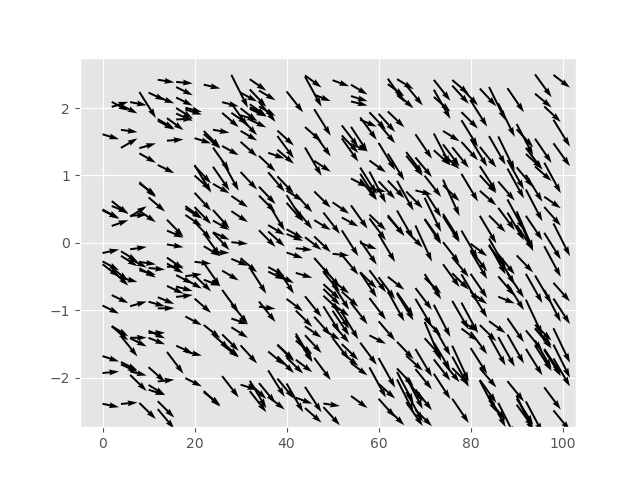
\includegraphics[width=0.45\linewidth]{figure/hs_dynamic2.png}\label{fig:hstateVector}}\hspace{5mm}
%     \subfigure[Visualization of the change of $\mu(t;e_i)$ in StackOverflow dataset. ]{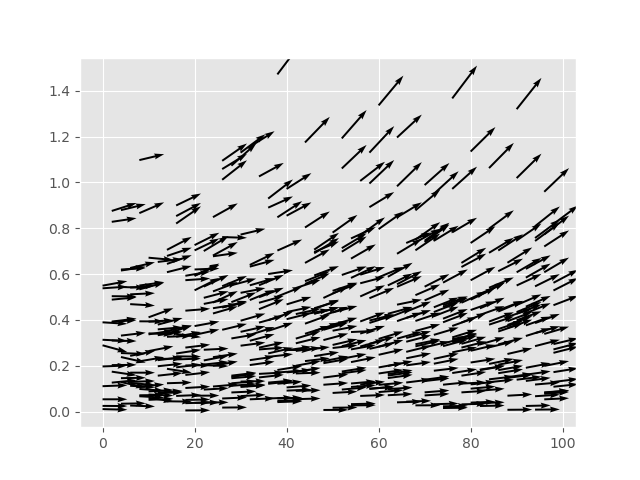
\includegraphics[width=0.45\linewidth]{figure/intensity_dynamic.png}\label{fig:muVector}}
%     \caption{Visualization of vector fields. a) is a vector field of the hidden state and b) is the vector field of $\mu(t;e_i)$. The length of the arrow represents the magnitude.}
%     \label{fig:vectorfields}
% \end{figure}
% % \vspace*{3in}

% \subsection{Visualization of Continuous Dynamics}
\begin{figure}[!h]
    \centering
    \subfigure[Visualization of $\mu(t;e_i)$ trained using MOOC.]
    {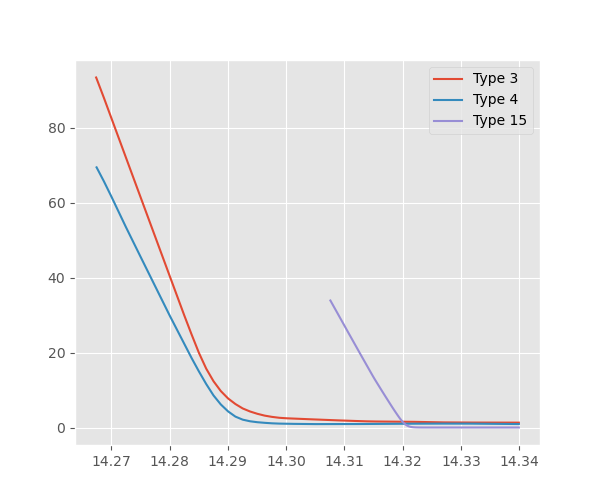
\includegraphics[height = 0.4\textwidth]{figure/mooc_inten.png}}
    \hfill
    \subfigure[\raggedright $\hat{f}(t;e_{i})$ trained using in MOOC.]
    {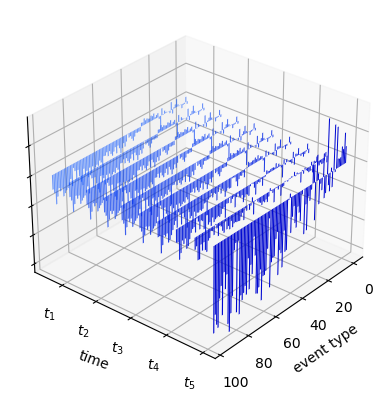
\includegraphics[height = 0.4\textwidth]
    {figure/mook_fk_14.png}}

    % \vspace{-0.3cm}
    \subfigure[$\mu(t;e_i)$ trained using Reddit.]
    {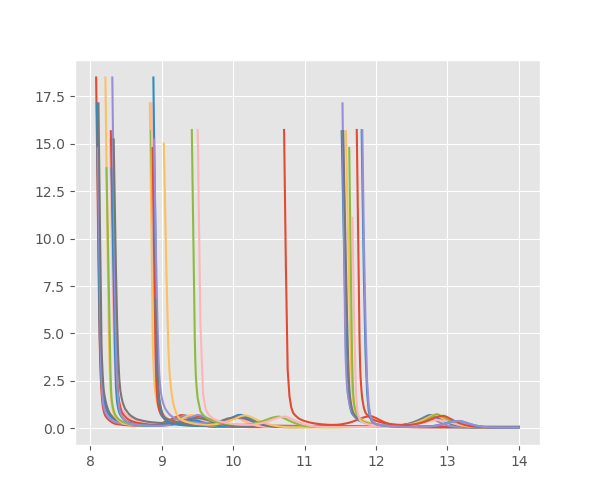
\includegraphics[height = 0.4\textwidth]{figure/reddit_inten.png}}
    \hfill
    \subfigure[\raggedright $\hat{f}(t;e_{i})$ trained on Reddit dataset.]
    {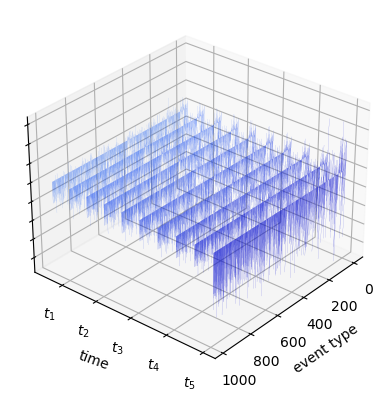
\includegraphics[height = 0.4\textwidth]
    {figure/reddit_fk_148.png}}
    \caption{Visualization of dynamics of $\mu$ and $\hat{f}$ in benchmark dataset. (a) is a visualization of ground intensity trained on MOOC dataset, (b) is a visualization of $\hat{f}(t;e_i)$ changing through time trained using MOOC dataset, (c) is a visualization of ground intensity trained on Reddit dataset, and (d) is a visualization of $\hat{f}(t;e_i)$ changing through time trained using Reddit dataset.}
\end{figure}

\begin{figure}[p] \ContinuedFloat
    \vspace{-10cm}
    % \vspace{-.3cm}
    \subfigure[Visualization of $\mu(t;e_i)$ trained using SO.]
    {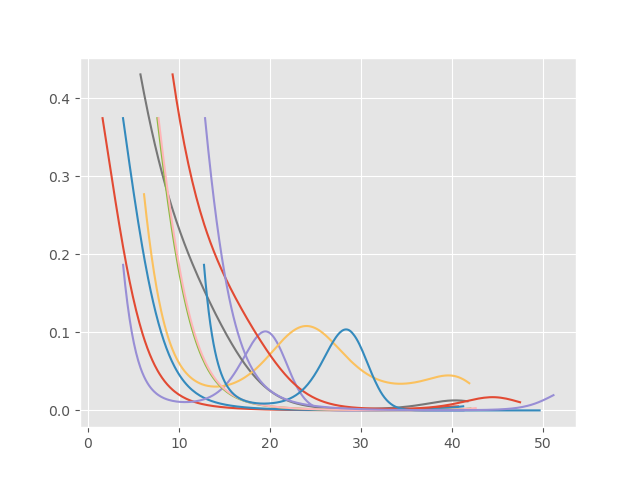
\includegraphics[height = 0.4\textwidth]{figure/SO_int.png}}
    \hfill
    \subfigure[\raggedright Visualization of $\hat{f}(t;e_{i})$ in MIMIC.]
    {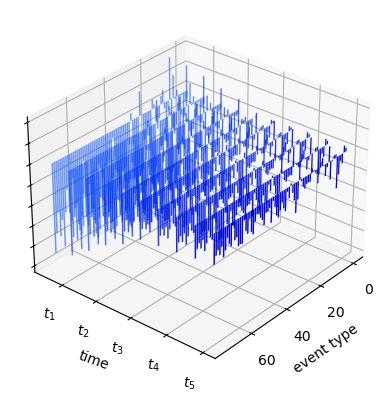
\includegraphics[height = 0.4\textwidth]{figure/mimic_fk_10.png}}
    \caption{Visualization of dynamics of $\mu$ and $\hat{f}$ in benchmark dataset. (a) shows dynamics of ground intensity trained using Stack Overflow dataset, and (b) shows $\hat{f}(t; e_i)$ changing through time trained using MIMIC-II dataset.}
    \label{fig:mooc}
\end{figure}
\clearpage

